\chapter{How To}
\label{chapter:how-to}

\section{Setup}
\label{sec:setup}
This \LaTeX\xspace template uses \texttt{BibLaTeX} and \texttt{Biber}. This StackExchange post\footnote{\url{https://tex.stackexchange.com/questions/154751/biblatex-with-biber-configuring-my-editor-to-avoid-undefined-citations}} explains how to setup your IDE accordingly. Additionally, this post\footnote{\url{https://tex.stackexchange.com/questions/25701/bibtex-vs-biber-and-biblatex-vs-natbib}} justifies why this setup is superior to \texttt{BibTeX} and \texttt{natbib}.

\section{Citations}
\label{sec:citations}
Let's see citations in action. The template uses \textit{authoryear} citation style, you can change it if you want.\\
A helpful \texttt{BibLaTeX} cheat sheet can be found here\footnote{\url{http://tug.ctan.org/info/biblatex-cheatsheet/biblatex-cheatsheet.pdf}}.\\
I prefer to explicitly denote which kind of citations I use. So, the most important commands are \textit{\textbackslash textcite} that is used for text cites, e.g., \textcite{bordes_translating_2013}, \textit{\textbackslash parencite} is used to cite with parentheses \parencite{bordes_translating_2013}. Multiple citations can be obtained with the plural form \textit{\textbackslash parencites} or \textit{\textbackslash textcites}, e.g. \parencites[e.g.][]{cauchy_methode_1847}{bordes_translating_2013}{nickel_review_2016}.\\
For direct citations, you can use the \texttt{csquotes} package. E.g., \enquote{Lorem ipsum \textelp{} dolor sit amet}.

\section{Acronyms}
\label{sec:acronyms}
Acronyms are handled easily. Short -- \acs{KG}, long -- \acl{KG}, full -- \acf{KG}, same for plural -- \acsp{KG}, \aclp{KG}, \acfp{KG} --- or simply \ac{KG}. Here, I also prefer to be explicit.

\section{Floats}
\label{sec:floats}
At this point, just some general advice:
\begin{enumerate}
	\item You can have separate captions for a single float: A full caption directly at the float and a shorter version for the table of contents, e.g., in Table \ref{tab:average-ensemble} the formatting of the table is only explained below the table, not in the table list at the beginning of the document.
	\item \textit{\textbackslash FloatBarrier} from the \texttt{placeins} package is awesome to place your floats. It literally is a barrier for your floats.
\end{enumerate}

\section{Tables}
\label{sec:tables}
The template uses \texttt{booktabs} for beautiful tables. Table \ref{tab:average-ensemble} is an example for a table that contains multiple tabulars. Table \ref{tab:single-hyperparameters} is a side-by-side table. Note the use of \textit{\textbackslash toprule}, \textit{\textbackslash midrule}, and \textit{\textbackslash bottomrule}. Table \ref{tab:kb-construction} shows another example that makes use of fancy superscript symbols.\\
\begin{table}[h]
	\centering
	\subfloat[Pre-training and no fine-tuning.]{
		\centering
		\begin{tabular}{lllll} \toprule
			Models				&	\acs{MR}	&	\acs{MRR}		&	hits@10			&	hits@1			\\
			\midrule
			\textsc{R+D}		&	276			&	0.258			&	0.420			&	0.179			\\
			\textsc{R+C}		&	378			&	0.246			&	0.405			&	0.167			\\
			\textsc{R+T}		&	253			&	0.264			&	0.423			&	0.185			\\
			\textsc{D+C}		&	200			&	0.293			&	0.481			&	0.200			\\
			\textsc{D+T}		&	204			&	0.317			&	0.484			&	\textbf{0.233}	\\
			\textsc{C+T}		&	281			&	0.305			&	0.478			&	0.218			\\
			\textsc{R+D+C}		&	265			&	0.269			&	0.437			&	0.186			\\
			\textsc{R+D+T}		&	212			&	0.284			&	0.450			&	0.202			\\
			\textsc{R+C+T}		&	238			&	0.277			&	0.441			&	0.195			\\
			\textsc{D+C+T}		&	\textbf{191}&	\textbf{0.321}	&	\textbf{0.494}	&	\textbf{0.233}	\\
			\textsc{R+D+C+T}	&	205			&	0.292			&	0.461			&	0.207			\\
			\bottomrule
		\end{tabular}
		\label{tab:average-ensemble-pre-no-fine}
	}\\
	\subfloat[Pre-training and fine-tuning.]{
		\centering
		\begin{tabular}{lllll} \toprule
			Models				&	\acs{MR}		&	\acs{MRR}		&	hits@10			&	hits@1			\\
			\midrule            
			\textsc{D+C+T-mb}	&	329				&	\textbf{0.312}	&	\textbf{0.501}	&	\textbf{0.217}	\\
			\textsc{D+C-l}		&	\textbf{178}	&	0.306			&	0.494			&	0.213			\\
			\bottomrule
		\end{tabular}
		\label{tab:average-ensemble-pre-fine}
	}\\
	\subfloat[No pre-training and fine-tuning.]{
		\centering
		\begin{tabular}{lllll} \toprule
			Models				&	\acs{MR}		&	\acs{MRR}		&	hits@10			&	hits@1			\\
			\midrule                                 
			\textsc{D+C-mb}		&	310				&	\textbf{0.288}	&	\textbf{0.480}	&	\textbf{0.193}	\\
			\textsc{D+C-l}		&	\textbf{259}	&	0.275			&	0.457			&	0.185			\\
			\bottomrule
		\end{tabular}
		\label{tab:average-ensemble-no-pre-fine}
	}
	\caption[Link prediction results for the \textsc{Average} ensemble.]{Link prediction results for the \textsc{Average} ensemble. Best-performing entries marked \textbf{bold}. Model names are abbreviated by their first character.}
	\label{tab:average-ensemble}
\end{table}

\begin{table}
	\centering
	\subfloat[Margin-based loss function.]{
		\begin{tabular}{lllllll}\toprule
			Model					&	$h$	&	$\alpha$	&	$\eta$	&	$\gamma$	&	$\lambda$\\
			\midrule            
			\textsc{Rescal}			&	100	&	0.5			&	1		&	8			&	0.1		\\
			\textsc{DistMult}		&	200	&	0.1			&	5		&	4			&	-		\\
			\textsc{ComplEx}		&	150	&	0.01		&	5		&	2			&	-		\\
			\textsc{TransE-$L_1$}	&	150	&	0.05		&	10		&	2			&	-		\\
			\bottomrule
		\end{tabular}
	}
	\hfill
	\subfloat[Logistic loss function.]{
		\begin{tabular}{lllllll}\toprule
			Model					&	$h$	&	$\alpha$	&	$\eta$	\\
			\midrule            
			\textsc{DistMult}		&	150	&	0.05		&	5		\\
			\textsc{ComplEx}		&	150	&	0.05		&	5		\\
			\textsc{TransE-$L_2^2$}	&	150	&	0.05		&	10		\\
			\bottomrule
			\\
		\end{tabular}
	}
	\caption{Best-performing hyperparameter settings for individual models.}
	\label{tab:single-hyperparameters}
\end{table}

\begin{table}
	\centering
	\begin{tabular}{lllll} \toprule
		Approach & Accuracy & Scalability & Schema & Example \\
		\midrule
		Curated & Very high & Very low & Yes & WordNet\textsuperscript{*} \\
		Collaborative & High & Low & Yes & Freebase\textsuperscript{$\dagger$} \\
		Semistructured & High & High & Yes & DBPedia\textsuperscript{$\ddagger$} \\
		Unstructured & Low & Very high & Yes & Knowledge Vault\textsuperscript{$\mathsection$} \\
		Unstructured & Low & Very high & No & CORE\textsuperscript{$\mathparagraph$} \\
		\bottomrule
	\end{tabular}
	\caption[Comparison of \acs{KB} construction approaches.]{Comparison of \acs{KB} construction approaches. Citations: (*) \textcite{miller_wordnet:_1995}, ($\dagger$) \textcite{bollacker_freebase:_2008}, ($\ddagger$) \textcite{auer_dbpedia:_2007}, ($\mathsection$) \textcite{dong_knowledge_2014}, ($\mathparagraph$) \textcite{petroni_core:_2015}.}
	\label{tab:kb-construction}
\end{table}
\FloatBarrier

\section{Algorithms}
\label{sec:algorithms}
Algorithms in pseudocode can be realized with the \texttt{algorithm} and \texttt{algpseudocode} packages as in the example of Algorithm \ref{alg:minibatch-sgd}.

\begin{algorithm}
	\caption{Minibatch \acl{SGD}}
	\label{alg:minibatch-sgd}
	\begin{algorithmic}[1]
		\Require Training data $K^{train}$
		\Require Initial parameters $\Theta$
		\Require Minibatch size $b$
		\Require Number of negatives $\eta$
		\While {stopping criterion not met}
			\For{$i = 1 .. \vert K^{train}\vert/b$}
				\State \textsl{// Sample a minibatch of positive triples without replacement}
				\State $K^{train}_i \gets$ \Call{sample}{$K^{train}$, $b$}
				\State \textsl{// Sample $\eta$ negative triples for each $x \in K^{train}_i$}
				\State $K_b \gets$ \Call{sample}{$K^{train}_i$, $\eta$}
				\State Update $\Theta$ w.r.t. $L(K_b; \Theta)$
			\EndFor
		\EndWhile
	\end{algorithmic}

\end{algorithm}

\section{Listings or Code}
\label{sec:listings}
A listings example of the \texttt{listings} package is depicted in Listing \ref{lst:distmult} that shows C++ code. Can be made more colorful, but I prefer to stay clean and simple.

\lstset{caption={Example implementation of \textsc{DistMult}.}, label={lst:distmult}}
\begin{lstlisting}
virtual double score(Triple &t)  {
	return (E->col(t.subject).array()*R->col(t.relation).array()*E->col(t.object).array()).sum();
}
virtual void gradient(Triple& t, double scale) {
	sub = R->col(t.relation).array()*E->col(t.object).array();
	rel = E->col(t.subject).array()*E->col(t.object).array();
	obj = R->col(t.relation).array()*E->col(t.subject).array();
	dE->add(t.subject, sub*scale);
	dR->add(t.relation, rel*scale);
	add(t.object, obj*scale);
}
\end{lstlisting}

\section{Figures}
\label{sec:figures}
Figure \ref{fig:hyperparameter-sensitivity-02} shows an example of a figure. It uses \textit{*.eps} figures to achieve a high resolution.

\begin{figure}[h]
	\centering
		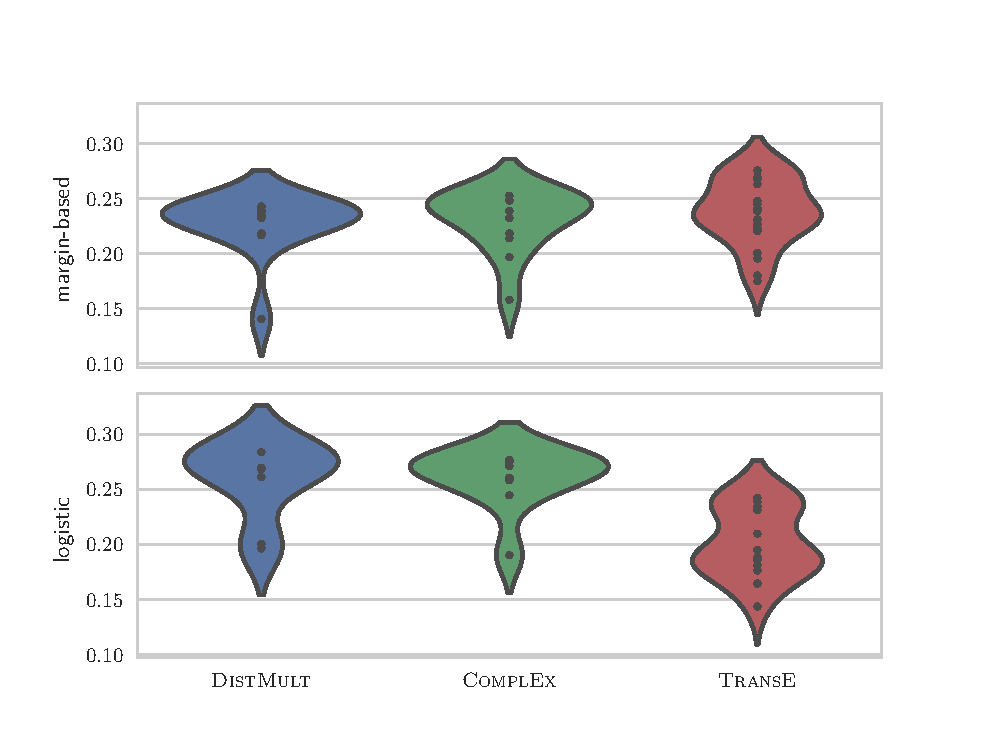
\includegraphics[width=\textwidth]{./img/hyperparameter-sensitivity.eps}
	\caption{Kernel density estimation plot of the \acs{MRR} metric for different hyperparameter settings.}
	\label{fig:hyperparameter-sensitivity-02}
\end{figure}

\section{Graphs and Drawings}
\label{sec:graphs}
Figure \ref{fig:sample-knowledge-graph} shows an example that uses the \texttt{tikz} package to render a sophisticated graph.

\begin{figure}
	\begin{tikzpicture}[entity/.style={circle, draw=black, minimum size=9mm, blur shadow, fill=white}, relation/.style={midway, fill=white}]
		\node[entity, label=below:\small \textsc{Ian McKellen}] (IMK) at (0,0) {};
		\node[entity, label=above:\small \textsc{Gandalf}] (Gandalf) at (0,3) {};
		\node[entity, label=below:\small \textsc{Lord of the Rings}] (LotR) at (3.5,0) {};
		\node[entity, label=above:\small \textsc{Fantasy}] (Fantasy) at (5,3) {};
		\node[entity, label=below:\small \textsc{Harry Potter}] (HP) at (6.5,0) {};
		\node[entity, label=below:\small \textsc{Alan Rickman}] (AR) at (10,0) {};
		\node[entity, label=above:\small \textsc{Snape}] (Snape) at (10,3) {};

		\draw[-{Latex[length=3mm]}] (IMK) -> (Gandalf) node[relation]{\footnotesize \textsc{played}};
		\draw[-{Latex[length=3mm]}] (AR) -- (Snape) node[relation]{\footnotesize \textsc{played}};
		\draw[-{Latex[length=3mm]}] (Gandalf) -- (LotR) node[relation]{\footnotesize \textsc{characterIn}};
		\draw[-{Latex[length=3mm]}] (Snape) -- (HP) node[relation]{\footnotesize \textsc{characterIn}};
		\draw[-{Latex[length=3mm]}] (LotR) -- (Fantasy) node[relation]{\footnotesize \textsc{genre}};
		\draw[-{Latex[length=3mm]}] (HP) -- (Fantasy) node[relation]{\footnotesize \textsc{genre}};
		\draw[-{Latex[length=3mm]}] (IMK) -- (LotR) node[relation]{\footnotesize \textsc{starredIn}};
		\draw[-{Latex[length=3mm]}] (AR) -- (HP) node[relation]{\footnotesize \textsc{starredIn}};
	\end{tikzpicture}
	\caption[Sample knowledge graph.]{Sample knowledge graph. Nodes represent entities, edges represent existing relations between entities. Adapted from \textcite{nickel_review_2016}.}
	\label{fig:sample-knowledge-graph}
\end{figure}

\section{Equations}
\label{sec:equations}
Equations can be aligned:
\begin{align*}
	1 + 1	&= 2\\
	3			&= 1 + 2
\end{align*}
Different cases:
\[
	y =	\begin{cases}
				0 & \text{if } x < 0\\
				x & \text{otherwise}
			\end{cases}
\]

\section{Todo Notes}
\label{sec:todo-notes}
Sometimes it is useful to take down some notes of what you plan to do. Especially, if you let someone proof read your thesis. The \texttt{todonotes} package is helpful for that purpose\todo{This is a side note.}. It has side notes as well as inline notes.\\
\todo[inline]{This is an inline note.}